%\documentclass[10pt]{beamer}
%\usetheme{amcg}
%\usepackage{subfigure}

%\begin{document}

\section{Lock--exchange}

\begin{frame}
  \frametitle{The lock--exchange}
  \begin{itemize}
  \item Flat bottomed tank, separated into two partitions by a barrier.
  \item Each half is filled with fluids of different density (temperature).
  \item The barrier is removed, and the denser fluid collapses under the lighter.
  \item The mesh changes in time as the dynamics evolves. 
  \end{itemize}

  \begin{figure}
    \centering
    \includegraphics[width=0.45\textwidth]{./lock_exchange/le_basic_0_T}
    \caption{Lock-exchange initial temperature distribution.  Blue labels dense fluid, and red lighter.}
  \end{figure}
\end{frame}

\begin{frame}
  \frametitle{The lock--exchange}
  \begin{figure}[ht]
    \centering
    % For some reason tex4ht doesn't like these images.
    \subfigure[$t = 0\,$s]{\includegraphics[width=0.45\textwidth]{./lock_exchange/le_basic_0_T}}
    \subfigure[$t = 0\,$s]{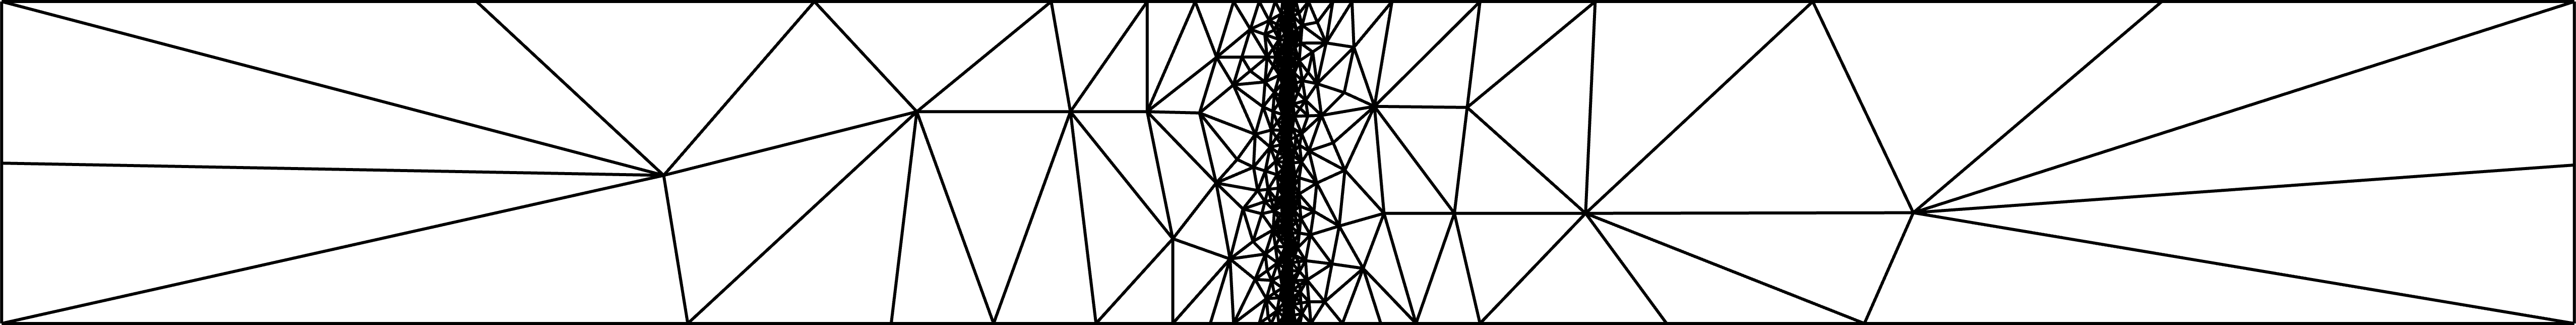
\includegraphics[width=0.45\textwidth]{./lock_exchange/le_basic_0_mesh_nice}} \\
    \subfigure[$t = 12.475\,$s]{\includegraphics[width=0.45\textwidth]{./lock_exchange/le_basic_10_T}}
    \subfigure[$t = 12.475\,$s]{\includegraphics[width=0.45\textwidth]{./lock_exchange/le_basic_10_mesh}} \\
    \subfigure[$t = 37.475\,$s]{\includegraphics[width=0.45\textwidth]{./lock_exchange/le_basic_30_T}}
    \subfigure[$t = 37.475\,$s]{\includegraphics[width=0.45\textwidth]{./lock_exchange/le_basic_30_mesh}}
    \caption{Lock-exchange temperature distribution (colour) with meshes, over time ($t$).}
  \end{figure}
\end{frame}
 
\begin{frame}
  \frametitle{The lock--exchange, diagnostics}
  \begin{itemize}
  \item Front speed (or Froude number).
  \item Mixing indicated by domain fractions of fluid in specified temperature classes.
  \end{itemize}

  \begin{figure}
    \centering
    \includegraphics[width=0.5\textwidth]{./lock_exchange/mixing}
    \caption{Time evolution of fraction of domain that contains fluid in three temperature classes. Blue: cold, red: warm, green: mixed}
  \end{figure}
\end{frame} 

\begin{frame}
  \frametitle{The lock--exchange, exercises}
  \begin{itemize}
  \item Experiment with the adaptivity options.
  \item Try adding some detectors to visualise the particle trajectories.
  \end{itemize}
\end{frame}

%\end{document}
